\documentclass{ximera}

\title{Linear Algebra}

\begin{document}
\begin{abstract}
  MIT OCW Linear Algebra Title Page
\end{abstract}\maketitle

\begin{center}
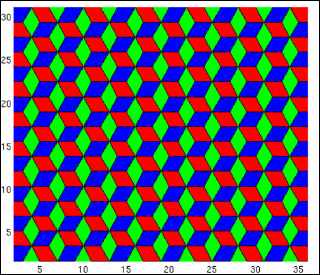
\includegraphics{Main.jpg}
\end{center}
\noindent
\textbf{Course Description}
\par
\noindent
This course covers matrix theory and linear algebra, emphasizing topics useful in other disciplines such as physics, economics and social sciences, natural sciences, and engineering.
\par
\noindent
\textbf{Course Format}
\par
\noindent
This course has been designed for independent study. It provides everything you will need to understand the concepts covered in the course. The materials include:
\par
\noindent
\textbf{Credits}
This course is a conversion of the MIT Linear Algebra class by Professor Gilbert Strang to Ximeria. Source from: \\
\url{http://ocw.mit.edu/courses/mathematics/18-06sc-linear-algebra-fall-2011/}
\end{document}
